\documentclass[]{article}
\usepackage{units}
\usepackage{cite}
\usepackage{array}
\usepackage{subfigure}
\usepackage{graphicx}
\usepackage{amsmath}
\usepackage{amssymb}
\usepackage{mathptmx}
%\usepackage{table}
%\usepackage{pslatex}
\usepackage{epsfig}
\usepackage{color}
\usepackage[normalem]{ulem}
\usepackage{wasysym}
\usepackage{fancyhdr}
\usepackage{multirow}
\usepackage{gensymb}

%opening
\title{Role of Haptics in Reduction of Cognitive Workload in Teleoperations}


\begin{document}

\maketitle


\section{Introduction}


  The transmission of force perception from a real (physical) or virtual object to an operator who may be in a remote location has significance in virtual reality (VR) and telerobotic operation \cite{galambos2012vibrotactile}. Haptic feedback is critical to allow a user to intuitively perceive and understand a distant or inaccessible environment even with visual feedback \cite{bark2013vivo}. In the absence of imagery, the sense of touch is more vital since it is often the only readily available and easily understood somatosensory feedback in robotic and virtual reality applications. An example of this is during robotic surgery where poor or occluded visibility is common with endoscopic cameras \cite{bouzit2002rutgers}.
  
  
  Arguably, force is one of the first contact events felt by humans.  The state of the art in force feedback systems involves real-time interaction between users present in remote locations to physically touch each other through actual force and pressure. A two-way communication can be established between these operators by projecting a floating silhouette of their counterpart and rendering this interaction in real-time through haptic feedback, making the users who are present in isolated locations to perceive this interaction as actual physical touch \cite{makino2016haptoclone}.


  However, it is extremely difficult to replicate and render force feedback accurately and with precise localization. These force feedback technologies often suffer from many shortcomings like robustness, latency, control issues and low availability of user friendly interfaces \cite{galambos2012vibrotactile} \cite{wagner2005mechanisms}. Flexible, light weight devices that are easy to use and can deliver haptic feedback with high spatial precision and intensity will be game- changing technologies, as they can have applications in a variety of fields especially where presence of humans is difficult and unlikely \cite{wagner2005mechanisms} \cite{nagendran2015symmetric}. Haptic feedback provides supplementary information to aid and abet the information obtained from other sensory modalities of audio and vision, allowing operators to intuitively understand an object’s properties situated at a remote and isolated location \cite{bark2013vivo}. 


  To address these shortcomings, we have designed and fabricated haptic gloves that are lightweight, flexible and capable of delivering haptic information with high spatial precision and intensity. Using a sensory substitution approach to transform pressure characteristics to vibratory stimuli has helped in reduction of size and bulkiness of a haptic device \cite{makino2016haptoclone}. However, a vibrotactile feedback strategy is limited by actuator size and a desire for flexibility, which restricts the number of actuation (sensing) points. This reduces spatial precision and range of stimulus presentation. 


  Visual augmentation is a phenomenon in which a user views a real world environment directly or indirectly while supplementing or ‘augmenting’ this environment with computer based sensory inputs such as graphics, imagery, sound or videos. In contrast to virtual reality where an artificial world is simulated around the operator, augmented reality (AR) allows digital manipulation and interaction with real world and environment, making this technology more relatable and relevant \cite{fernandes2015remembering}. In the field of telerobotics, visual augmentation allows resourcefulness and several modelling approaches as real world data can be used in real time to make human-robots cooperation more adaptive and intelligent \cite{fu2015towards}. Once considered as science fiction, AR has helped tremendously in remote operations of semiautomatic systems which when coupled with haptic feedback allows intuitive understanding of remote environment aiding human-computer-robot cooperation \cite{sheridan1995teleoperation}. In medicine, this technology has tremendous applications especially in developing minimally invasive and highly safe surgical tools to provide real time 3D computer generated anatomical environment augmented on a surgical platform \cite{haouchine2013image}. 


  However, AR has many drawbacks, especially in the fields that are heavily dependent on the field of view of the operation procedure. Dextrous telerobotic systems suffer from latency issues as robotic manipulators are controlled by the movements performed by remote operators which are very often misrepresented and misclassified. The newer generations of this technology should invest in more user friendly interfaces that represent the real anatomy of the object under consideration and allow for quick transition, synchronised with the movement of the deployed robot through varied environments \cite{berman2015design}. 


  In the field of disaster recovery, tele-manipulation and space exploration, AR and haptics can create an immersive and real environment with sensory feedback, giving the users present far away from the site to carry search and rescue operations effectively without having to be physically present at the location \cite{mollet2009virtual}.

\section{Methodology}

The experimental setup consists of an eye tracking system, EEG data acquisition system and a fully immersive virtual reality CAVE system. The subjects will also be asked to wear haptic feedback gloves that provide vibration feedback upon stimulation.

\subsection{Electroencephalogram}
For accurate measurement of surface brain activity, the EEG system consisting of an EEG cap with a 64-channel EEG amplifier connected to a data acquisition system is used. ASA Lab software is used to check for the impedance of the electrodes. EEG and EOG activity is recorded by the amplifier at 256 samples per second (ANT Neuro data aquisition system). 

\subsection{Virtual Reality}
A cave automatic virtual environment (CAVE) is an alternative immersive environment. The CAVE uses projectors to create a virtual world on three to six walls of a cube, the cube could be of different size and shape. The ability to interact with and control a robot in a natural and intuitive manner is not well developed. Our platform will permit a user inside the master system to communicate with and operate a robot with a set of gesture language. The simulated environment that CAVE produces the avatar of robots for users. The use of gestures has long been a desired feature of most computer interactive tools. Our gesture recognition approach will allow users to perform tasks with multiple levels of natural body language. Our work focuses on developing a gesture control languages that aims to send control event at a more convenient way. The experimental setup consists of a CAVE system with 4 screens, and Advanced Realtime Tracking system. Our method tracks multiple levels of gesture data by gathering both ART tracking data and camera stream input. 

\begin{figure}
	\centering
	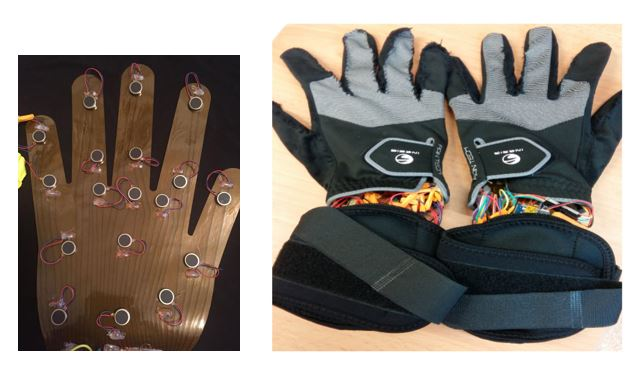
\includegraphics[width=0.8\textwidth]{Capture.jpg}
	\caption{Left: Actuator integration on Flexible PCB to provide localised feedback. Right: Haptic Gloves used for experimentation}
	
\end{figure}

\subsection{Haptic glove}
A vibro-tactile haptic glove was developed using eccentric rotating mass (ERM) motors (as seen in Fig 1). The glove has the capability of rendering spatial touch information with amplitude modulation. The high-density glove has 18 vibratory eccentric rotating mass actuators. The actuator locations were selected to deliver haptic feedback at the most used and sensitive areas on the palm-side of the hand during exploratory procedures. The control box is placed at the wrist location. The vibration intensity and their activation is controlled wirelessly through a graphical user interface (GUI) that is designed to send custom stimulation patterns. The GUI enables single and multiple actuator activation with amplitude modulation for intensity control.  In near-field operation the latency is low permitting real-time feedback. The control box consists of two pulse width modulation (PWM) drivers and one Arduino microcontroller. The computer transmitting an encoded stimulation signal received by the control box initiates the communication pathway. This signal is sent to a microcontroller for actuation. In addition, the control box contains a power source for the system. 



\subsection{Experimental Protocol}

For measurement of mental workload, a pick and place task was simulated in the CAVE. The subjects were asked to grasp a virtually simulated object from a basket and place it into another basket with their hand positions being tracked by markers integrated with the advanced real-time tracking system. A clustering algorithm was developed to map the users hand in 3D space. The experimental protocol was designed as follows:

\begin{itemize}
	\item Training session: 20 minutes
	   \begin{itemize}
	    \item 10 minutes session pick and place experiment without haptic feedback (baseline).
	    \item 10 minutes session pick and place experiment with haptic feedback.
	   \end{itemize}
	\item Testing session: 20 minutes with and without haptic feedback.
\end{itemize}

Behavioural parameters like time taken for object transfer and number of objects were evaluated.
\begin{figure}
	\centering
	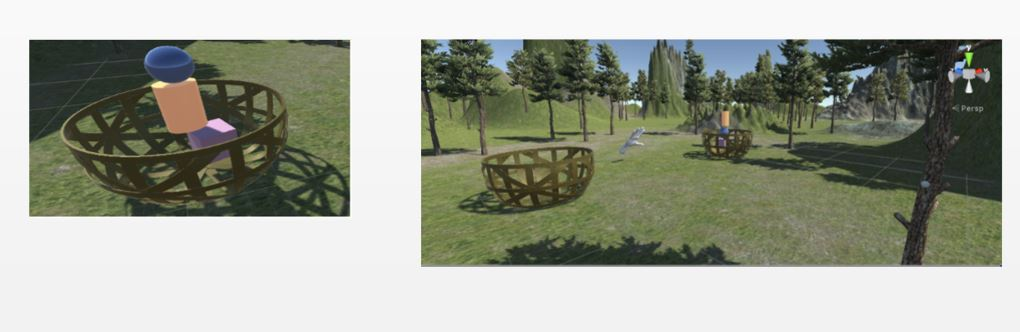
\includegraphics[width=1.0\textwidth]{Capture1.jpg}
	\caption{Left: Virtual objects used in the simulation. Right: Experimental task}
	
\end{figure}
\\\\\\\\\\\\
\bibliography{ref}
\bibliographystyle{unsrt}

\end{document}
